%DIF PREAMBLE EXTENSION ADDED BY LATEXDIFF
%DIF UNDERLINE PREAMBLE %DIF PREAMBLE
\RequirePackage[normalem]{ulem} %DIF PREAMBLE
\RequirePackage{color}\definecolor{RED}{rgb}{1,0,0}\definecolor{BLUE}{rgb}{0,0,1} %DIF PREAMBLE
\providecommand{\DIFadd}[1]{{\protect\color{blue}\uwave{#1}}} %DIF PREAMBLE
\providecommand{\DIFdel}[1]{{\protect\color{red}\sout{#1}}}                      %DIF PREAMBLE
%DIF SAFE PREAMBLE %DIF PREAMBLE
\providecommand{\DIFaddbegin}{} %DIF PREAMBLE
\providecommand{\DIFaddend}{} %DIF PREAMBLE
\providecommand{\DIFdelbegin}{} %DIF PREAMBLE
\providecommand{\DIFdelend}{} %DIF PREAMBLE
%DIF FLOATSAFE PREAMBLE %DIF PREAMBLE
\providecommand{\DIFaddFL}[1]{\DIFadd{#1}} %DIF PREAMBLE
\providecommand{\DIFdelFL}[1]{\DIFdel{#1}} %DIF PREAMBLE
\providecommand{\DIFaddbeginFL}{} %DIF PREAMBLE
\providecommand{\DIFaddendFL}{} %DIF PREAMBLE
\providecommand{\DIFdelbeginFL}{} %DIF PREAMBLE
\providecommand{\DIFdelendFL}{} %DIF PREAMBLE
%DIF END PREAMBLE EXTENSION ADDED BY LATEXDIFF

%\documentclass{sigplanconf}
%\nocaptionrule

% \documentclass[twocolumn,9pt]{article}
% \documentclass[twocolumn,10pt]{acm_proc_article-sp}

% \documentclass{acm_proc_article-sp}
\documentclass[9pt]{sigplanconf}

\date{} % \vspace*{-0.2in}}

% Make sure to put back 

\newcommand{\punt}[1]{}

\punt{

Notes from Daan Leijen:
}

\usepackage{endnotes,xspace}

\newcommand{\footnotenonumber}[1]{{\def\thempfn{}\footnotetext{\small #1}}}
\usepackage[normalem]{ulem}
\usepackage{graphicx}

\usepackage{mathptmx} % rm & math
\usepackage[scaled=0.90]{helvet} % ss
\usepackage{courier} % tt
% \normalfont
\usepackage[T1]{fontenc}

% \usepackage{lmodern}
% \usepackage{times}
\usepackage{subfigure}
\usepackage{url}
\urlstyle{rm}
\usepackage[
      colorlinks=false,    %no frame around URL
      urlcolor=black,    %no colors
      menucolor=black,    %no colors
      linkcolor=black,    %no colors
      pagecolor=black,    %no colors
]{hyperref}

\usepackage{color}
\usepackage{listings}
\usepackage{amsmath}
\usepackage{amsfonts}
\usepackage{amssymb}
\usepackage{comment} 
\usepackage{setspace}
\singlespacing
%\onehalfspacing
\newtheorem{thm}{Theorem}
\newtheorem{prop}[thm]{Proposition}
\newtheorem{cor}[thm]{Corollary}
\newtheorem{lem}[thm]{Lemma}
\newtheorem{defn}[thm]{Definition}

\newcommand{\cfunction}[1]{{\bf \tt #1}}
\newcommand{\malloc}{\cfunction{malloc}}
\newcommand{\realloc}{\cfunction{realloc}}
\newcommand{\free}{\cfunction{free}}
\newcommand{\madvise}{\cfunction{madvise}}
\newcommand{\brk}{\cfunction{brk}}
\newcommand{\sbrk}{\cfunction{sbrk}}
\newcommand{\mmap}{\cfunction{mmap}}
\newcommand{\munmap}{\cfunction{munmap}}
\newcommand{\mprotect}{\cfunction{mprotect}}
\newcommand{\mlock}{\cfunction{mlock}}

\hyphenation{app-li-ca-tion}
\hyphenation{Die-Hard}
\hyphenation{Ar-chi-pe-la-go}
\hyphenation{buf-fer}
\hyphenation{D-threads}
\hyphenation{Heap-Layers}
\hyphenation{wait-Token}
\hyphenation{mul-ti-threa-ded}
\hyphenation{me-m-ory}

\hyphenation{pthread-create}
\hyphenation{pthread-self}
\hyphenation{pthread-mutex-lock}
\hyphenation{pthread-mutex-unlock}

\newcommand{\dthreads}{{\scshape Dthreads}}
\newcommand{\Dthreads}{{\scshape Dthreads}}
\newcommand{\doubletake}{{\scshape DoubleTake}}
\newcommand{\DoubleTake}{{\scshape DoubleTake}}
\newcommand{\stopgap}{{\scshape DoubleTake}}
\newcommand{\Stopgap}{{\scshape DoubleTake}}
\newcommand{\StopGap}{{\scshape DoubleTake}}
\newcommand{\Sheriff}{{\scshape Sheriff}}
\newcommand{\sheriff}{{\scshape Sheriff}}
\newcommand{\Grace}{{\scshape Grace}}
\newcommand{\grace}{{\scshape Grace}}
\newcommand{\SheriffProtect}{\textsc{Sheriff-Protect}}
\newcommand{\sheriffProtect}{\textsc{Sheriff-Protect}}
\newcommand{\sheriffprotect}{\textsc{Sheriff-Protect}}
\newcommand{\SheriffDetect}{\textsc{Sheriff-Detect}}
\newcommand{\sheriffDetect}{\textsc{Sheriff-Detect}}
\newcommand{\sheriffdetect}{\textsc{Sheriff-Detect}}
\newcommand{\pthreads}{\texttt{pthreads}}

\definecolor{lightgray}{rgb}{.9,.9,.9}
\definecolor{darkgray}{rgb}{.4,.4,.4}
\definecolor{purple}{rgb}{0.65, 0.12, 0.82}

\lstdefinelanguage{c++threads}[]{c++}{
  morekeywords={pthread_create,pthread_join},
  keywordstyle=\color{blue}\bfseries,
  ndkeywords={class, export, boolean, throw, implements, import, this},
  ndkeywordstyle=\color{darkgray}\bfseries,
  identifierstyle=\color{black},
  sensitive=false,
  comment=[l]{//},
  morecomment=[s]{/*}{*/},
  commentstyle=\color{purple}\ttfamily,
  stringstyle=\color{red}\ttfamily,
  morestring=[b]',
  morestring=[b]"
}
\lstset{
   language=c++threads,
   backgroundcolor=\color{lightgray},
   extendedchars=true,
   basicstyle=\footnotesize\ttfamily,
   showstringspaces=false,
   showspaces=false,
   numbers=none,
   numberstyle=\footnotesize,
   numbersep=9pt,
   tabsize=2,
   breaklines=true,
   showtabs=false,
   captionpos=b
}
%\lstset{language=c++threads, basicstyle=\ttfamily\scriptsize,frame=trbl,tabsize=4} % ,numbers=left,numberstyle=\tiny}

\definecolor{Gray}{cmyk}{0,0,0,0.5}

\begin{document}

\CopyrightYear{2014}
\copyrightdata{XXX-X-XXXXX-XXX-X/XX/XX}

\title{{\huge \bf \doubletake{}}: Evidence-Based Dynamic Analysis}
% Efficiently and Precisely Locating Buffer Overflows}

% \authorinfo{\emph{authorship list removed for anonymity}}

%\punt{
\authorinfo{Tongping~Liu \and Charlie~Curtsinger \and Emery~D.~Berger}
{School of Computer Science \\
University of Massachusetts Amherst \\
Amherst, MA 01003 \\
{\{tonyliu,charlie,emery\}@cs.umass.edu}
}

\punt{
\numberofauthors{1}
\author{
\alignauthor Tongping~Liu and Emery~D.~Berger \\
\affaddr{Department of Computer Science} \\
\affaddr{University of Massachusetts, Amherst} \\
\affaddr{Amherst, MA 01003} \\
\email{\{tonyliu,emery\}@cs.umass.edu} \\
}
}

\maketitle

\begin{comment}
\end{comment}

\begin{abstract}
Dynamic analysis can be helpful for debugging, but is often too
expensive to use in deployed applications. We introduce evidence-based
dynamic analysis, an approach that enables extremely lightweight
analyses for an important class of errors: those that can be forced to
leave evidence of their existence. Evidence-based dynamic analysis lets
execution proceed at full speed until the end of an epoch. It then
examines program state to find evidence that an error occurred at some
time during that epoch. If so, execution is rolled back and
re-execution proceeds with instrumentation activated to pinpoint the
error. We present \doubletake{}, a prototype evidence-based dynamic
analysis framework. We demonstrate its generality by building analyses
to find buffer overflows, memory use-after-free errors, and memory
leaks. \doubletake{} is precise and efficient: its buffer overflow
analysis runs with just 2\% overhead on average, making it the fastest
such system to date.



\end{abstract}

%  Language-based approaches require programmers to write their code in specialized languages. 


\punt{
\category{D.1.3}{Programming Techniques}{Concurrent Programming--Parallel Programming}
\category{D.2.5}{Software Engineering}{Testing and Debugging--Debugging Aids}

\terms
Design, Reliability, Performance

\keywords
Buffer Overflow, Detection 
}


%%%%%%%%%%%%%%%%%%%%%%%%%%%%%%%%%%%%%%%%%%%%%%%%%%%%%%%%%%%%%%%%%%%%%%%%%%%%%%%%%%%%%%%%%%%%%
%%%%%%%%%%%%%%%%%%%%%%%%%%%%%%%%%%%%%%%%%%%%%%%%%%%%%%%%%%%%%%%%%%%%%%%%%%%%%%%%%%%%%%%%%%%%%

\section{Introduction}
% Dynamic analysis
% Super-duper awesome

Dynamic analysis tools are widely used to find bugs in
applications. They are popular among programmers because of their
precision---for many analyses, they report no false positives---and
can pinpoint the exact location of errors, down to the individual line
of code.

Perhaps the most prominent and widely used dynamic analysis tool for
C/C++ binaries is Valgrind~\cite{overflow:valgrind}. Valgrind's most
popular use case, via its default tool, memcheck, is to check memory
errors, including buffer overflows, use-after-free errors, and
memory leaks.

Unfortunately, while these dynamic analysis tools are useful, they are
often expensive. Using Valgrind typically slows down applications by
10-100$\times$. Faster dynamic analysis frameworks exist for finding
particular errors, but all impose substantial overheads. Google's
AddressSanitizer, for example, detects buffer overflows and
use-after-free errors, but slows applications by around 30\%. Precise
memory leak detectors that identify the point at which objects are
leaked remain far more expensive.

Because of their overhead, dynamic analysis tools are only used during
debugging. However, they are limited by definition to the executions
that they have seen. The fact that using these tools in deployed
applications is not practical means that errors that could
have been found trivially instead require painstaking debugging
later.

This paper presents a new approach that enables extremely lightweight
dynamic analysis for an important class of errors. These errors share
a monotonicity property: when an error happens, evidence that it
happened either remains or grows in memory so that it can be recovered at a
later point. When this evidence is not naturally occurring, it is
often possible to ``plant'' evidence via what we call \emph{tripwires}
to ensure later detection. An example tripwire is a random value, also
known as a ``canary'', placed in unallocated space between heap
objects~\cite{StackGuard}. A corrupted canary is incontrovertible 
evidence that a buffer overflow occurred at some time in the past.

We present an approach called \emph{evidence-based dynamic analysis} that is based on the
following key insight: by combining checkpointing with evidence
gathering, it is possible to let applications run at full speed in the
common case (no errors). If we discover evidence of an error, we can
go back and re-execute the program with instrumentation activated to
find the exact cause of the error.

We present a prototype evidence-based dynamic analysis framework called \doubletake{}. \doubletake{} performs its checkpoints only at
irrevocable system calls, amortizing the cost of checkpoint
collection. Each checkpoint saves the contents of the stack,
globals, registers, and the heap. If it finds evidence of an error at
the next system call or after a segmentation violation, \doubletake{}
re-executes the application from the most recent checkpoint. During
re-execution, it triggers instrumentation to let it precisely locate
the source of the error. For buffer overflows, \doubletake{} sets hardware watchpoints on the tripwire
memory locations that were found to be corrupted. During re-execution,
\doubletake{} can pinpoint exactly the point where the buffer overflow
occurred.

We implement \doubletake{} as a drop-in library that can either be
linked directly with the application under analysis, or which can be
activated by setting an environment variable (\texttt{LD\_PRELOAD} on
Unix systems) to dynamically load \doubletake{} before execution. No
re-compilation or availability of source code is required. This
approach makes \doubletake{} as convenient to use as Valgrind.

We have built three different analyses using \doubletake{}: buffer
overflow detection, use-after-free detection, and memory leak
detection. All of these analyses run without any false positives,
precisely pinpoint the error location, and operate
with \emph{extremely} low overhead: for example, with \doubletake{},
buffer overflow analysis operates with just 2\% overhead on average,
making it the fastest overflow detector to date and thus feasible to
use in deployed scenarios.

\subsection*{Contributions}

The contributions of this paper are the following:

\begin{enumerate}

\item It introduces \emph{evidence-based} dynamic analysis, a new analysis technique that combines checkpointing with evidence gathering and instrumented replay to enable precise error detection with extremely low overhead.

\item It presents \doubletake{}, a framework that implements evidence-based dynamic analyses for C/C++ programs: its analyses (detecting buffer overflows, use-after-frees, and memory leaks) are the fastest reported to date.

\end{enumerate}


%\subsection{Outline}
%This paper talks about those related works in next section. Section 3 discusses specific mechanisms 
%used by \doubletake{}. Section 4 describes some implementation details worth noting. 
%Section 5 evaluates the performance and effectiveness of \doubletake{} and Section 6
%discusses some problems and extending possibilities of \doubletake{}.
%Section 7 concludes this paper. 


\section{Overview}
Figure~\ref{fig:nondeterminism} shows an example multithreaded program that, because of data races, non-deterministically produces the outputs ``1,0,'' ``0,1,'' and ``1,1.''  The order of instructions are changed from one execution to the other, resulting in these nondeterministic outputs. Using \dthreads{}, this program will \emph{deterministically} produce the same output-``1,1'' . Although this output can be a undesired one, the fact that results are always reproducible would make it easy for developers to reproduce and locate data races inside parallel programs.

\begin{figure}[h]
{\centering
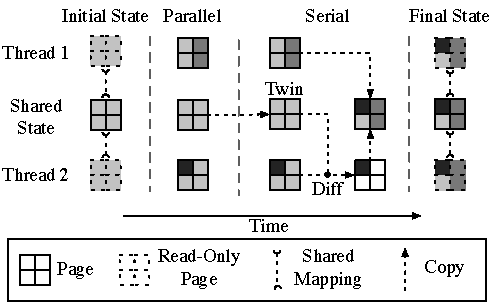
\includegraphics[width=6in]{dthreads/figure/architecture-diagram}
\caption{An overview of \dthreads{} execution.\label{fig:architecture}}
}
\end{figure}

\dthreads{} employs the following mechanisms to ensure the deterministic execution, illustrated by Figure~\ref{fig:architecture}: 

\textbf{Isolated Memory Access:} In \dthreads{}, threads are actually running as separate processes with private and shared views of memory, which is based on the \sheriff{} framework. Because processes have separate address spaces, \dthreads{} can isolate executions of different ``threads''. \dthreads{} uses this isolation mechanism to control the visibility of memory state, so that the updates made by a thread can not be seen by other threads if those updates are not committed explicitly to the shared mapping. By doing this, we guarantee that each ``thread'' can operate independently until synchronization points. Implementation of this is discussed in depth in Section~\ref{sec:threadsasprocs}.

\textbf{Deterministic Memory Commit:} 
Multithreading programs use shared memory for communication, thus \dthreads{} must propagate a thread's changes to be seen by other threads. To guarantee determinism, \dthreads{} should publish updates of different threads in a deterministic order at deterministic points.

\dthreads{} actually commits the changes of a thread to the shared state in sequence at synchronization points. These points includes thread creation and exit; mutex lock and unlock; condition variable wait and signal; posix sigwait and signal; and barrier waits. Commits are ordered using a global ``token'' that is passed from one thread to the next; a thread can only commit when it holds the token.  The token-passing protocol is described in Section~\ref{sec:schedule} and the implementation of synchronization primitives is described in Section~\ref{sec:synchronization}.

\dthreads{} relies on the twinning and diffing mechanism to find out local changes of different threads, which has been discussed in Section~\ref{sec:twinning-and-diffing}. 

\textbf{Deterministic Synchronization:}
There is no deterministic guarantee on synchronizations under existing operating systems. Thus, \dthreads{} re-implements the full range of pthreads synchronization primitives and discusses  them in details in Section~\ref{sec:synchronization}. 

\hspace{1em} \\
\noindent
\textbf{Fixing the data race example} \\
About the example program in Figure~\ref{fig:nondeterminism},  \dthreads{} effectively isolates the execution from each thread until it completes, and then orders updates from different threads by thread creation time using a deterministic last-writer-wins protocol.

In the beginning of every execution, thread 1 and thread 2 have the same view of shared state, with a = 0 and b = 0. Because changes by one thread to the value of a or b will not be made visible to the other until this thread exits, both checks on two threads on line 2 will be true. Thread 1 sets the value of a to 1, and thread 2 sets the value of b to 1. These threads then commit their updates to the shared state and exit, with thread 1 always committing before thread 2. The main thread then should always prints “1, 1” on every execution.

This determinism not only enables record-and-replay and replicated execution, but also effectively converts Heisenbugs into “Bohr” bugs, making them reproducible. In addition, \dthreads{} optionally reports any conflicting updates due to racy writes, further simplifying debugging.


\section{Applications}
\label{sec:applications}

\subsection{Shared Mechanisms}
Before the description of different applications, we listed some shared mechanisms that are used by one or multiple applications. 

\subsubsection{Canary}
\label{sec:canary}
Canary was first proposed by StackGuard~\cite{StackGuard} to find stack smashing problems by placing a canary word before the return address on stack. Those attempts to overwrite the return address should corrupt the canary word at first. Canaries are borrowed to detect buffer overflow ~\cite{overflow:purify}. They are initialized to a special value in the beginning so that modifications of those values indicates the problems. Detection tools can place canary values anywhere in heap memory. \doubletake{} introduces a bitmap to track the locations of canary values, and can check for canaries that have been overwritten. Buffer overflow detection places canary values between heap objects to detect out-of-bounds writes, and use-after-free detection fills freed objects with canaries to detect writes through dangling pointers.

\subsubsection{Watchpoints}
\label{sec:watchpoints}
Watch point mechanism relies on hardware debug registers to monitor memory accesses on specific addresses. Previous work has used this mechanism for their specific targets ~\cite{fastboundschecking, Kivati}. The main target of debug registers is to support software debuggers, e.g. gdb. A small number of watchpoints are available on modern architectures (four on x86). Each watchpoint can be configured to pause program execution when a specific byte or word of memory is accessed. \doubletake{} allows detection tools to set hardware watchpoints before re-execution. Heap Overflow detection tool can use watchpoints to find the instruction(s) responsible for overwriting a canary value.

\subsection{Applications}
\label{sec:applications}

\doubletake{} implements three important applications based on its lightweight dynamic analysis framework. Those applications are implemented in a best-effort way to show the efficiency of our framework. They are not targeted for a complete and novel solution, thus most of mechanisms are borrowed from previous work. 

\begin{figure}[!t]
\begin{center}
\includegraphics[width=3.3in]{doubletake/figure/buffer-overflow-diagram}
\end{center}
\caption{Heap organization used to provide evidence of buffer overflow errors. Object headers and unrequested space within allocated objects are filled with canaries; a corrupted canary indicates an overflow occurred.
\label{fig:buffer-overflow}}
\end{figure}

\begin{figure}[!t]
\begin{center}
\includegraphics[width=3.3in]{doubletake/figure/dangling-pointer-diagram}
\end{center}
\caption{Evidence-based detection of dangling pointer (use-after-free) errors. Freed objects are deferred in a quarantine in FIFO order and filled with canaries. A corrupted canary indicates that a write was performed after an object was freed.
\label{fig:dangling-pointer}}
\end{figure}


\subsubsection{Detection of Heap Buffer Overflows}
\label{sec:overflow}
Buffer overflows occurs when a program writes outside of the range of an allocated object. Buffer overflows can greatly affect the reliability and security of a program. 

\paragraph{Detection.}
To detect heap buffer overflows, \DoubleTake{} puts canaries before and after actual heap objects, which is described in Figure~\ref{fig:buffer-overflow}. This method is borrowed from previous work~\cite{overflow:lbc, AddressSanitizer}.
All heap objects of \doubletake{} are managed by power of two size, adding two words for canaries (16 bytes) for each heap object. For an allocation size not power of two size (a non-aligned object), \doubletake{} rounds it up to the next power of two size class, putting byte-based canaries and word-based canaries immediately after this object. This approach lets \doubletake{} catch overflows as small as one byte. 

Detection happens in the following scenario. At memory deallocation, \doubletake{} checks buffer overflows only for non-aligned objects, with size different with the power of two class. At the end of each epoch, \doubletake{} verifies integrities of all canaries by traversing the bitmap, which marks the placement of canaries and discussed in Section~\ref{sec:canaries}.  Corrupted canaries indicates heap buffer overflows. 

\paragraph{Re-execution.}
\label{sec:overflowreport}
When a program is found to have heap overflows, \doubletake{} rolls back the execution to the most recent checkpoint and re-executes this program.
To precisely identifying instructions responsible for a buffer overflow, \doubletake{} installs a watch point at the address of a corrupted canary before re-execution. When the program is re-executed, any instruction that writes to this address will trigger a debug trap (resulting in a SIGTRAP signal). \doubletake{} then reports the exact call site of trapped instructions, acquired by calling \texttt{backtrace} function. To further help programmer, \doubletake{} can also report the allocation site of an overflowed heap object. 
  
\subsubsection{Detection of Memory Leak}
\label{sec:leak}
Heap memory is leaked when it becomes inaccessible without being freed. Memory leak can greatly reduce the performance and availability of programs, which makes it one of common classes of reported bugs.

\paragraph{Detection.}
\doubletake{} detects memory leak using the same marking mechanism as conservative garbage collection ~\cite{Wilson:1992:UGC:645648.664824}. \doubletake{} marks the reachability of all heap objects: whether a heap object is reachable from the globals, the stack, and registers. Any unreachable object that has not been freed must be leaked. 

In order to compute the reachability from globals, stack, and registers, \doubletake{} starts to put all possible pointers, any eight-byte aligned value falling into the range of the heap, into a work queue. Then \doubletake{} checks all values in the queue using a breadth-first search algorithm: for each value, \doubletake{} verifies whether this value is a valid address inside a heap object; If this valid object is still non-reachable (not checked before), \doubletake{} marks it as reachable and also put all possible pointers inside this object into the work queue. After this step, this value is removed from the work queue. \doubletake{} stops when there is no value in the work queue any more. In this time, all heap objects which is reachable should have been marked. 

After the marking phase, \doubletake{} traverses the whole heap to find leaked objects, those un-reachable non-freed objects. To simplify the marking and checking phase, the status of an object, whether it is freed or reachable are marked in the object header. During this traverse, \doubletake{} recovers the status of every object to un-reachable. \doubletake{} also adds all leaked objects into a global hash table, where each leaked object also keeps information of its starting address and size. 

\paragraph{Re-execution.}
\label{sec:leakreport}
\doubletake{} uses re-execution to find allocation sites for all leaked heap objects. Re-execution proceeds as normal, with an added check in each \texttt{malloc()} function call. When a memory allocation matches the actual size and address of any leaked heap object, 
\doubletake{} reports its call stack, obtaining by using \texttt{backtrace} 
functions of \texttt{glibc} library. 

\subsubsection{Detection of Use-after-free Errors}
\label{sec:danglingpointer}
Memory use-after-free errors occur when an application continues to use a pointer after its corresponding object has been deallocated.
Writing to a freed memory can overwrite the contents of lived objects, leading to unexpected behavior.  

\paragraph{Detection.}
To detect memory use-after-free errors, 
\doubletake{} firstly delays memory re-usage of all freed objects 
by putting them into a quarantine list, same as AddressSanitizer does ~\cite{AddressSanitizer}. 
Those objects in the quarantine list are actually returned back
to the program heap when the total size of freed objects in the quarantine list are larger then a pre-defined threshold or the quarantine list is full.

In order to find evidence of memory use-after-free problems, 
\doubletake{} fills the first 128 bytes of an object, which can be adjustable, with canaries. 

Those canaries are checked before an object is returned back to the program heap or in the end of an epoch. Same as detection of buffer overflows, 
a corrupted canary indicates a use-after-free memory error and must be reported to user. 

\paragraph{Re-execution}
When a program has use-after-free memory errors, \doubletake{} re-executes this program to find out the allocation and deallocation site of corresponding objects and those instructions actually writing them.
%It is possible that multiple instructions can access an object after deallocation.  

To obtain an object's call site of allocation and deallocation, 
\doubletake{} checks starting address of each object during every memory allocation and deallocation. If an object has the same address as those use-after-free objects, its corresponding allocation/deallocation site are saved. To find out those instructions writting a freed object, 
\doubletake{} installs hardware watch points on those violating addresses, which shares the same mechanism as overflow detection.
\doubletake{} reports an use-after-free error, with its allocation site and deallocation site, in order to help programmers locate a memory use-after-free error. 

\section{Implementation}
\label{sec:implementation}

\doubletake{} is implemented as a library and can be linked directly to programs, or can be injected into unmodified binaries by setting the \texttt{LD\_PRELOAD} environment variable on Linux.

At startup, \doubletake{} begins a new epoch. The epoch continues until the program issues an \emph{irrevocable} system call (see Section~\ref{sec:syscalls} for details). Before this call is issued, \doubletake{} scans program state for evidence of errors. The details of this scan are presented in Section~\ref{sec:applications}.

If no errors are found \doubletake{} ends the epoch, issues the irrevocable system call, and begins a new epoch. If any detection tools have found evidence of an error, \doubletake{} enters re-execution mode. The remainder of this section describes the implementation of \doubletake{}'s core functionality.

\subsection{Epoch Start}
\label{sec:implementation/start}

At the beginning of each epoch, \doubletake{} takes a snapshot of program state. \doubletake{} saves all writable memory (stack, heap, and globals) from the main program and any linked libraries, and saves register state of each thread with the \texttt{getcontext} function. Read-only memory does not need to be saved. To identify all writable mapped memory, \doubletake{} reads the Linux \texttt{/proc/self/map} file. \doubletake{} also saves file positions of all open files. This lets programs issue \texttt{read} and \texttt{write} system calls without ending the current epoch. \doubletake{} uses the saved memory state and file offset to ``undo'' these calls if the epoch needs to be re-executed when an error is found.

%%%%%%%%%%%%%%%%%%%%%%%%%%%

\subsection{Normal Execution}
\label{sec:implementation/normalexecution}

Once a snapshot has been saved, \doubletake{} lets the program execute normally. Most program operations proceed normally, but \doubletake{} interposes on heap allocations and system calls in order to set tripwires and support re-execution.

%%%%%%%%%%%%%%

\subsubsection*{System Calls}
\label{sec:syscalls}
\begin{table}[t]
	\centering
	\small
	\renewcommand{\arraystretch}{1.5}
	\begin{tabular}{l|p{6cm}}
		\textbf{Category} & \textbf{Functions} \\
		\hline
		
		Repeatable		& \texttt{getpid}, \texttt{sleep}, \texttt{pause}\\
		
		Recordable		& \texttt{mmap}, \texttt{gettimeofday}, \texttt{time}, 
						  \texttt{clone} , \texttt{open}\\
		
		Revocable		& \texttt{write}, \texttt{read} \\
		
		Deferrable		& \texttt{close}, \texttt{munmap} \\
		
		Irrevocable		& \texttt{fork}, \texttt{exec}, \texttt{exit}, \texttt{lseek}, \texttt{pipe}, \texttt{flock}, \texttt{socket related system calls}\\
	\end{tabular}
	\caption{System calls handled by \doubletake{}. All unlisted system calls are conservatively treated as irrevocable, and will end the current epoch. Section~\ref{sec:syscalls} describes how \doubletake{} handles calls in each category.\label{table:syscalls}}
\end{table}

\doubletake{} ends each epoch when the program attempts to issue an irrevocable system call. However, most system calls can safely be re-executed or undone prior to re-execution. 

\doubletake{} breaks system calls into five categories, shown in Table~\ref{table:syscalls}. System calls could be intercepted using \texttt{ptrace}, but this would add unacceptable overhead during normal execution. Instead, \doubletake{} interposes on all library functions that may issue system calls.

%%%%%%%

\emph{Repeatable system calls} do not modify system state, and return the same result during normal execution and re-execution. No special handling is required for these calls.

\begin{figure*}[ht!]
	\begin{center}
		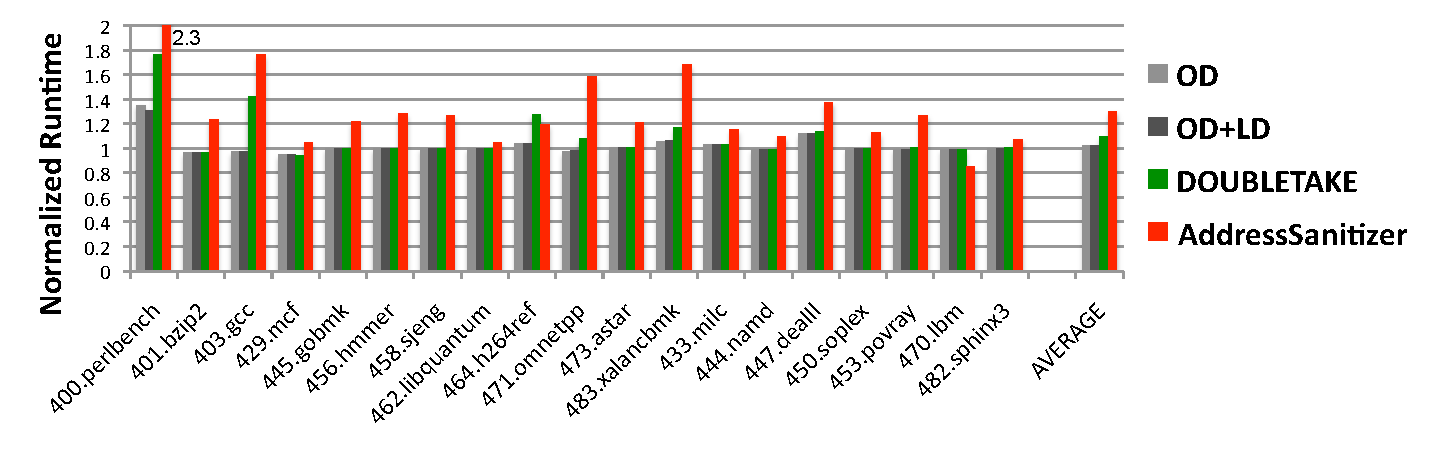
\includegraphics[width=6.5in]{figure/perf}
	\end{center}
	\caption{Runtime overhead of \doubletake{} (OD = Buffer Overflow Detection, LD = Leak Detection, \doubletake{} = all three detections enabled) and AddressSanitizer, normalized to each benchmark's original execution time. 
%Overhead for Valgrind is reported in Table~\ref{table:valgrind} because the results do not fit on this graph.
\label{fig:perf}}
\end{figure*}

%%%%%%%

\emph{Recordable system calls} may return different results if they are re-executed. \doubletake{} records the result of these system calls during normal execution, and returns the saved result during re-execution. Some recordable system calls, such as \texttt{mmap}, change the state of underlying operating system. Memory mapped with a call to \texttt{mmap} is left mapped for the entire epoch's re-execution; this is safe because the program cannot access this memory until the point at which the \texttt{mmap} call is replayed.

\emph{Revocable system calls} modify system state, but \doubletake{} can save the original state beforehand and restore it prior to re-execution. Most file I/O fall into this category.

For example, \texttt{write} modifies file contents, \doubletake{} can write the same content during re-execution. \texttt{write} also changes the current file position, which \doubletake{} restores to the saved file position using \texttt{lseek} prior to re-execution. \doubletake{} saves all file descriptors of opened files in a hash table at the beginning of each epoch. In addition, \doubletake{} must save stream contents returned by \texttt{fread}. Calls to \texttt{read} and \texttt{write}  on normal files, which can be identified by check the hash map, don't need to be handled. But those calls on socket files are treated as irrevocable system calls.
	
\emph{Deferrable system calls} will irrevocably change program state, but can safely be delayed until the end of the current epoch. \doubletake{} delays all calls to \texttt{munmap} and \texttt{close}, and executes these system calls before exiting or starting a new epoch.
	
\emph{Irrevocable system calls} change internally-visible program state, and cannot be undone. \doubletake{} must end the current epoch before these system calls are allowed to proceed. Note that for \doubletake{}, the meaning of ``irrevocable'' is different from that used in transactional memory systems~\cite{Irrevocabletrans}. Unlike in transactions, we expect re-execution to be identical to the epoch's original execution. It is safe for system calls to affect externally-visible state as long as the effect on internal state can be hidden or undone.

Note that in the presence of multiple threads, an error may fail to appear in the re-execution because of data races (synchronization ordering is already tracked and replayed). \doubletake{} then re-executes the code in an attempt to reveal the error. If it fails to reveal the error on replay, \doubletake{} has effectively tolerated the error and continues execution.

%%%%%%%%%%%%%%

\subsubsection*{Multithreaded Support}
We have implemented support for multiple threads, but the recording and re-execution of thread synchronizations is not yet stable. \doubletake{} records the sequence of system calls and results separately for each thread.

Every mutex records the order of threads that acquire it, and condition variables record the order of thread wakeups. \doubletake{} does not enforce a total global order on lock acquisitions. Operations within a single thread are totally-ordered, and \doubletake{} enforces local order at each synchronization point. In the absence of data races, this is sufficient to ensure deterministic re-execution.

Calls to \texttt{pthread\_create} are recorded with the same mechanism as recordable system calls. When a new thread starts, \doubletake{} takes a snapshot of the thread's stack and registers to enable re-execution from the beginning of the thread's execution. As with synchronization operations, \doubletake{} logs thread creation order and enforces this order during re-execution. Calls to \texttt{pthread\_exit} are deferred until the end of the epoch. Because \texttt{pthread\_exit} is deferred, \texttt{pthread\_join} is effectively deferred as well.

%%%%%%%%%%%%%%

\subsubsection*{Heap Allocator}
\label{sec:heapallocator}

Heap allocators typically issue a large number of \texttt{mmap} or \texttt{sbrk} system calls, which would complicate \doubletake{}'s logging re-execution. \doubletake{} replaces the default heap with a fixed-size BiBOP-style allocator with per-thread subheaps and power-of-two size classes, built using Heap Layers~\cite{heaplayers}. \doubletake{}'s heap is completely deterministic, so no logging is required to ensure that allocations do not change during re-execution.

When an object is freed, the allocator checks which subheap it is allocated from. If the object comes from the freeing thread's subheap, the \texttt{free} call proceeds uninterrupted. If the object was originally allocated by a different thread, the \texttt{free} is deferred. When the epoch ends, each object whose \texttt{free} was deferred is returned to its source thread's freelist.

During replay, \doubletake{}'s heap allocator checks to see if the object being allocated or freed contains the address where an error was detected. If so, \doubletake{} calls the \texttt{backtrace()} function to obtain a call stack for the allocation and deallocation sites.

\doubletake{} lets error detection tools traverse the set of all allocated objects during error checking. Objects are marked as allocated in object headers, including a size of the \emph{requested size}, which may be less than the power-of-two size class for object. All three detection tools use this size during scanning.

\doubletake{} also maintains a bitmap to record the locations of heap canaries. The bitmap records every word of heap memory that contains a canary. \doubletake{} notifies the detection tool when any of the bytes do not contain canaries. Buffer overflow detection places canaries only outside the requested object size. Re-execution is only started if the detection tool finds that canaries between allocated objects have been overwritten.

%%%%%%%%%%%%%%

\subsubsection*{Epoch End}

The epoch ends when any thread issues an irrevocable system call. All other threads are notified with a signal. Once all threads have stopped, \doubletake{} checks the program state for errors. The application-specific error checks are described in Section~\ref{sec:applications}. If an error is found, \doubletake{} immediately switches to re-execution mode. If not, the runtime issues any deferred system calls and clears the logs for all recorded system calls.

%%%%%%%%%%%%%%%%%%%%%%%%%%%

\subsection{Re-Execution}
\label{sec:implementation/re-execution}

Before re-executing the current epoch, \doubletake{} must roll back program state. Restoring saved memory will overwrite the current stack, so \doubletake{} switches to a temporary stack during rollback. The saved state of all writable memory is copied back, and any revocable system calls are undone (see Section~\ref{sec:implementation/normalexecution} for details). Before restoring register state, \doubletake{} must allow detection tools to place watchpoints.

\subsubsection*{Watchpoints}
Debug registers are not accessible in user-mode, so \doubletake{} must use \texttt{ptrace} to set watchpoints. \doubletake{} forks a child process and attaches to it using \texttt{ptrace} to load watched addresses into the debug registers and enable the watchpoints.

Once watchpoints have been placed, \doubletake{} uses the \texttt{setcontext} call to restore register state and begin re-execution. During re-execution, \doubletake{} replays the saved results of system calls from the log collected during normal execution. All deferred system calls are converted to no-ops while the program is re-executing.

\subsection*{Synchronization Replay}
\doubletake{} enforces the recorded order of synchronization operations during re-execution. A thread can only acquire a mutex if it is the next thread in the acquisition log, regardless of whether the mutex is currently locked. \doubletake{} uses semaphores to wake threads from condition variables in the recorded order. When a condition variable is signaled, the signaling thread notifies next waking thread that it can resume. If this thread has not yet arrived at the condition variable, it will wake immediately after it arrives.


%\section{\doubletake{} for Multithreading Programs}
%\label{sec:multithreading}

This section describes the mulithreading support of \doubletake{}.
A thread is a basic execution unit from the point of view of underlying operating system. 
The order of an execution, greatly affecting memory usage, 
is highly depending on timing, synchronization order and internal scheduling algorithm.   
Thus, it is much more difficult to achieve the target of repeatable memory 
usage for multithreading programs, which is crucial to 
precisely detect buffer overflows or other memory errors.
This section first discusses how to handle epochs in multithreading programs.
After this, it describes the design of heap allocator, suitable for repeatable memory usage.
It then discusses how to handle thread creation and exits specially. 
In the end, it describes how to guarantee deterministic synchronization in the re-execution phase,
which is also crucial for repeatable memory usage.


\subsection{Overview}
\label{sec:mtoverview}

As described in Section~\ref{sec:overview}, \doubletake{} uses irrevocable system calls as 
boundaries for epochs for multithreading programs. 
To simplify description in the following sections, a thread encountering an irrevocalbe system call is 
called as the ``Triggering-Thread''. 

When encountering an irrevocable system call, this Triggering-Thread 
has to stop all existing threads so that all other threads are in a quiecent state, which
has been described in Section~\ref{sec:stopepoch}.
Then it performs memory checkings on the heap as described in Section~\ref{sec:epochend}. 
If there is no buffer overflow, it can perform this irrevocable system call and 
start a new epoch after this system call. 
Before waking up other threads, the Triggering-Thread takes a snapshot for the shared memory at first,
including the heap and globals. 
After a thread is waken up, it only needs to take a snapshot on its own state, 
including its stack and its hardware registers. 

If there are buffer overflows, the Triggering-Thread sets up the shared memory 
for all threads at first.
It recovers the heap and globals by copying from the saved snapshot. 
Then it can wake up other threads. 
However, if the Triggering-Thread is spawed newly in current epoch, 
it has to wait for its parent to start its execution. 

\subsubsection{Epoch}
\label{sec:stopepoch}

It is the duty of a Triggering-Thread to close an epoch.
Whenever this thread meets an irrevocable system call, it has to stop other threads.
\doubletake{} utilizes the ``signal'' mechanism to stop other threads asynchronously.
It signals other threads using SIGUSR2 signal when a thread is in a safe state. 
A thread is considered to be in a unsafe state before this thread finishs a snapshot for itself,
discussed in Section~\ref{sec:threadcreation}.
After sending out all signals, this thread is waiting on a internal conditional variable.
The Triggering-Thread only starts checking buffer overflows after all threads are in quiescence.

However, this SIGUSR2 signal can also be used by user programs. 
In order to differentiate this, \doubletake{} specifically marks on 
a shared flag before signalling so that signal handler can check this in the beginning. 
If this flag is marked, this signal is issued by \doubletake{}. Otherwise, it is issued by
a user program and we can call user registered program instead. 

When other threads receive the signal from the Triggering-Thread, 
they are waiting on an internal conditional variable for instructions from the Triggering-Thread:
it can move forward to next epoch or rollback.
It is worthy noting that inside signal handler we have to utilize a different lock that has not been
used by other places. Otherwise, it is easy to cause deadlock. 

\subsubsection{Customized Heap Allocator}
\label{sec:mtheap}
In order to achive the target of repeatable memory usage, the heap allocator must be designed 
carefully. \doubletake{} first borrows a ``per-thread-heap'' idea from Hoard~\cite{Hoard}. 
\doubletake{} keeps a 1-to-1 mapping between threads and sub-heaps of customized memory allocator. 
The total number of threads and sub-heaps are pre-defined. 
A thread can only allocate memory from its own sub-heap, 
where those sub-heaps can get the memory from a pre-allocated heap 
by allocating a huge block of memory each time. 
After a sub-heap gets a block of memory, its corresponding thread always owns all objects
of this block, called as ``owner'' of this block.
This surely can cause memory blowup problem resolved by Hoard. However, it is 
not the focus of \doubletake{}.   

The ``per-thread-heap'' idea is not enough to guarantee the repeatable memory usage. 
\doubletake{} imposes several additional rules besides this.
Firstly, when \doubletake{} acquires a block of memory from the global pre-allocated heap, it must 
acquire a lock at first, which is guaranteed to be deterministic according to mechanisms 
discussed in Section~\ref{sec:sync}.
This guarantee that every new blocks of each sub-heap is repeatable for re-execution. 
Secondly, when there is a memory deallocation, this freed object can only be returned back  
to its original owner in a safe state. 
If this memory deallocation is issued by the same thread as the owner, then this freed object
can be putted into the owner's free list and be utilized immediately. 
If this memory deallocation is issued by a different thread with the owner, 
which indicates a cross-thread communication,  
then this memory
deallocation are cached into a global list, which only issued in the end of this epoch after 
all threads has been stopped. 
By doing this, we can guarantee all memory usage inside an epoch is repeatable in re-execution phase.
 
\subsection{Thread Creation and Exit}
\label{sec:threadcreation}
Tracking creations and exits of threads is very important because of the following reasons.
First, \doubletake{} has to take snapshots for different threads in the beginning. 
Second, terminination of a thread invokes \texttt{munmap} system calls directly by \pthreads{}, which
can not be intercepted.  
Third, thread creation is considered as a synchronization and has to be recorded. 
Thus, \doubletake{} intercepts \texttt{pthread\_create} calls and changes its start routine 
to a customized function. 
In this customized function, \doubletake{} can record thread creation, take a snapshot and delay thread exit to the end of current epoch. 

\subsubsection{Normal Execution}

\doubletake{} makes \texttt{pthread\_create} to call its customized function as the start routine. 
In this start routine, \doubletake{} first puts this new thread into a global map, which maintains
status of all threads. 
Then it takes a snapshot for this new thread, including stack and hardware registers. 
After this, \doubletake{} can invoke the original routine to actually perform user-defined 
thread function. 

After this user-defined thread function finishes, the control flow returns back to \doubletake{}. 
Basically, \doubletake{} should check whether this thread's parent is joining on this thread or not. 
If this thread's parent is already waiting for its termination, it simply marks the status of 
this thread to be joined and wakes up the joining thread. 
If not, this thread can wait on a thread-private conditional variables. 
\doubletake{} delays a thread exit to the end of current epoch.

\subsubsection{Re-execution}
A thread is waiting for its turn to run if a thread is created in current epoch.    

\subsection{Thread Synchronizations}

\label{sec:sync}

Different order of thread synchronizations can lead to totally different memory uage. 
In order to guarantee deterministic replay of thread synchronizations, previous work
actually forces threads to do synchronizations in a global order and
recordes both lock and unlock operations ~\cite{TERN, PRES}. 
However, forcing a global order of synchronizations can greatly 
reduce parallelism and introduce significant performance overhead.
Also, it is unnecessary to record unlock order too.

Unlike previous approaches, \doubletake{} only records local orders of synchronizations.
Synchronizations on two different synchronization variables can be performaed
in parallel. From a thread's point of view, if a program do not have a race and
all synchronizations of a thread are repeated deterministically, then
\doubletake{} can guarantee memory usage of this thread, which also guarantees to 
repeat the same buffer overflows in re-execution phase. 
If a program do have a race, forcing a global order of synchronizations in the production 
run also can not completely avoid races. This also implies that a global order 
can not always guarantee determinstic memory uage.   
\doubletake{} prefers performance for racey programs, while relying on multiple re-executions 
to repeat buffer overflows if a program does have a race problem. 

\doubletake{} records the order of \texttt{pthread\_mutex\_lock}, conditional wakenup and
different signalling functions.
Signalling functions actually calls system calls, which are handled by the procedure discussed 
in Section~\ref{sec:inepoch}.
 Conditional wakenup is actually related to \texttt{pthread\_cond\_wait},
which actually includes conditional wait and conditional wakenup phases. 
Conditional wait atomically releases mutex and waits on corresponding conditional variable, while conditional wakenup actually locks corresponding mutex before returning. 
Thus, we can turn \texttt{pthread\_cond\_wait} to two operations, \texttt{pthread\_mutex\_unlock} and
\texttt{pthread\_mutex\_lock} correspondingly. So we only record the order of conditional wakenup in
production runs. 
 
\doubletake{} also provides an option to record the order of passing a specified barrier, which it is 
not necessary to do this by default.
It is noted that \doubletake{} do not record the order of unlock operations
and conditional signal operations.
It is totally unnecessary to record unlock operations since recording the order of actual 
lock aquiring operations is enough to guarantee a deterministic replay of critical sections.  
Conditional signal and broadcast operations are skiped for the same reason. 

%why two different synchronization is not important?
How to replay this?
How to handle nested locks? 
The replaying is considerred to be two steps: we first advance thread's entry when we met a .

Maybe pseudo code for this.
 
\subsubsection{Normal Execution}
In production runs, \doubletake{} intercepts all synchronizations and 
records orders of synchronizations, such as lock, conditional waken up and signals, 
based on different synchronization variables. 
It maintains a list for each synchronization variable and records synchronization
events on its corresponding list. 
In order to quickly locate its list when a synchronization is intercepted, \doubletake{}
utilizes original synchronization variables to store addresses of list and actual synchronization
variable. 

For a synchronization event like lock, \doubletake{} records the following information:
which thread issues this synchronization event; what is the result of this synchronization.
A naive implementation is to allocate memory from internal memory allocator every time. 
However, for some applications having significant amount of synchronizations,
memory allocations to record synchronization events contributes much performance overhead. 
For example, \texttt{fluidanimate} runs several times slower because of huge amounts
of synchronizations inside. \doubletake{} uses a pre-allocated list for those recordings. 
More specifically, each thread has a pre-allocated list in the beginning of an epoch. 
When a synchronization occurs on this thread, it can get an entry from this thread and 
record a synchronization event on this entry.
Since \doubletake{} always gets an entry from current thread issuing a synchronization,
there is no need to utilize a lock, which also helps reducing overhead. 
By doing this, \doubletake{} greatly reduce performance overhead of logging synchronization
events. For example, performance overhead of \texttt{fludidanimate} are reduced to around 40\%.

 
\subsubsection{Re-execution}
As described above, for a synchronization event in a thread,
\doubletake{} allocates an entry from current thread to record this synchronization event 
and inserted it into synchronization variable's corresponding list. 
This implies that a synchronization event belongs to two lists, 
a list for all synchronizations of this synchronization variable (SyncVariableList) and 
a list for all synchronizations in a thread (ThreadSyncList). 

Reproducing synchronizations involves in manipulating these two lists using 
{\it sempaphore replay}, similar to TERN ~\cite{TERN}.
We listed the pseudocode of ``lock'' of reproduction runs in Figure~\ref{fig:lockunlock}.
\doubletake{} assigns a semaphore for each thread and controls the order 
of synchronizations based on semaphores: in lock acquisitions, 
a thread waits on its semaphore and advances ThreadSyncList after this semaphore; 
In lock releases, a thread increments the semaphore of next thread on the same 
synchronization variable.
However, \doubletake{} only records local synchronization order, instead of global order,
synchronizations replaying of \doubletake{} is much more subtle.
In order to handle those unsuccessful lock acquisitions, \doubletake{} only waits for a semaphore 
if this lock is successfully acquired in the production run. 
Also, to support nesting locks, in lock acquisitions after {\it advanceThreadSyncList()}, 
\doubletake{} signals current thread if next event of this thread is already 
in its pending list, which means that this thread should have its turn.
For lock releases, \doubletake{} adds next event of SyncVariableList to corresponding thread's 
pending list if the event is not the first event of corresponding thread instead of incrementing
its semaphore directly. 
Since performance of reproduction runs is not the main focus, only occurring for those programs 
having buffer overflows, \doubletake{} are using the same lock for all lists' manipulations to
avoid races.  




%\section{Optimization}
%\input{optimization}

\section{Evaluation}
\begin{figure*}[htb]
{\centering
\tiny
\subfigure{\lstinputlisting[numbers=none,frame=none,boxpos=t]{predator/figure/linearregression.report}}
\caption{An example report by \Predator{} indicating false sharing in the linear\_regression benchmark.
\label{fig:lrreport}}
}
\end{figure*}



\label{sec:evaluation}

This section answers the following questions:
\begin{itemize}
\item
  How effective is \Predator{} at detecting and predicting false sharing?

\item
  What is \Predator{}'s overhead, in terms of execution time and memory ?

\item
  How sensitive is \Predator{} to different sampling rates?
 
\end{itemize}

\paragraph{Experimental Platform.} All evaluations are performed on a quiescent Intel Core 2 dual-processor system equipped with 
16GB RAM. Each processor is a 4-core 64-bit Intel Xeon running at 2.33 GHz, with a 4MB shared L2 cache and 32KB private L1 cache. The underlying operating system is an unmodified CentOS 5.5, running with Linux kernel version 2.6.18-194.17.1.el5. The glibc version is 2.5. 

\paragraph{Evaluated Applications.}
This paper evaluates two popular benchmark suites,
Phoenix (with large input) ~\cite{phoenix-hpca} and PARSEC (with simlarge input) ~\cite{parsec}. Even with unmodified LLVM-3.2, Facesim cannot be compiled successfully (having complaints on an undefined template) and Canneal aborts unexpectedly. Thus, these two benchmarks are excluded.
We also evaluate \Predator{} on six real applications, including MySQL, Boost, Memcached, aget, pbzip2 and pfscan.



\subsection{Detection and Prediction Effectiveness}
\label{sec:effective}

For every false sharing problem, \Predator{} reports source code information and detailed memory access information in order to help users fix those problems. Figure~\ref{fig:lrreport} shows an example for the linear\_regression benchmark. This report shows that the heap object starting with $0x40000038$ potentially causes a large number of cache invalidations. The call stack of allocation is provided to help locate culprits. In addition, \Predator{} also reports word-level access information of this object, which helps to identify where and how false sharing occurs. From that, we can know that it is a latent false sharing problem predicted by \Predator{}, since different threads are accessing different cache lines. 

\subsubsection{Benchmarks}
\label{sec:benchmarks}

\begin{table*}[!t]
{\centering\begin{tabular}{l|r|r|r|r|r}\hline
{\bf \small Benchmark} & {\bf \small Source Code} & {\bf \small New} & {\bf \small Without Prediction} &{\bf \small With Prediction} & {\bf \small Improvement} \\
\hline
\small \textbf{histogram} & {\small histogram-pthread.c:213} & \cmark{} &\cmark{} & \cmark{} & 46.22\%\\
\small \textbf{linear\_regression} & {\small linear\_regression-pthread.c:133} & & & \cmark{} & 1206.93\% \\
\small \textbf{reverse\_index} & {\small reverseindex-pthread.c:511} & & \cmark{} & \cmark{} & 0.09\%\\
\small \textbf{word\_count} & {\small word\_count-pthread.c:136} & & \cmark{} & \cmark{} & 0.14\%\\
\hline
\small \textbf{streamcluster} & {\small streamcluster.cpp:985} &  & \cmark{} & \cmark{} &7.52\% \\
\small \textbf{streamcluster} & {\small streamcluster.cpp:1907} & \cmark{} & \cmark{} & \cmark{} & 4.77\%\\
\hline
\end{tabular}
\caption{False sharing problems in the Phoenix and PARSEC benchmark suites. \label{table:detection}}
}
\end{table*}

Table~\ref{table:detection} provides detection results of two benchmark suites, Phoenix and PARSEC
The first column lists those programs with false sharing problems.  The second column shows precisely where the problem is. Because all discovered false sharing occurs inside heap objects, we show callsite source code information here.  The third column, ``New'', marks whether this false sharing was newly discovered by \Predator{}.  A checkmark in the following two columns indicates whether the false sharing was identified without
prediction and/or with prediction.  The final column, ``Improvement'', shows the performance improvement after fixing false sharing.
%The number is based on the average runtime of $10$ runs. 

As shown in the table, \Predator{} reveals two unknown false sharing problems. It is the first tool to detect the false sharing problems in histogram and in line $1908$ of streamcluster. 
In histogram, multiple threads simultaneously modify different locations of the same heap object, thread\_arg\_t. 
Padding this data structure fixes the false sharing problem and improves the performance by around 46\%. In streamcluster, multiple threads are simultaneously accessing and updating the same \texttt{bool} array, switch\_membership. Simply changing all elements of this array to a long type reduces the false sharing and improves the performance by about 4.7\%.

%, although it is not a complete fix of false sharing. 
%None of these two false sharing problems has been reported by previous tools.
Other false sharing problems were discovered by previous work~\cite{sheriff}. We do not see significant performance improvement for reverse\_index and word\_count benchmarks. They are reported here because the number of cache invalidations in these two programs reaches our predefined threshold.
Making the reporting threshold higher can avoid the report of those insignificant false sharing problems.
It is worth noting that these two benchmarks definitely have false sharing problems,
which can be confirmed by word-level information generated by \Predator{}. 

The streamcluster benchmark has another false sharing problem at line $985$. Different threads change the work\_mem object simultaneously. Authors of streamclsuter have already realized this problem and provide a CACHE\_LINE macro. Unfortunately, the default value of this macro is set to $32$ bytes, which is different from the actual cache line size of the experimental machine. By setting it to $64$ bytes instead, it achieves  performance improvement of about 7.5\%.

linear\_regression has a severe false sharing problem. Fixing it improves the performance by more than $12\times$. In this benchmark, different threads update their thread-specific locations inside the tid\_args object in a tight loop. According to the observation of Nanavati et al., this false sharing problem occurs when using clang and disappears when using gcc with the -O2 and -O3 optimization level~\cite{OSdetection}. But we observed a different result when using the clang-3.2 compiler and our custom memory allocator: the false sharing problem does not occur at all because the offset of the starting address of the potentially falsely-shared object and the start of cache line is 56 bytes (see Figure~\ref{fig:perfsensitive}). With prediction mechanism, \Predator{} detects this latent false sharing problem, exemplifying the necessity of a predictive detection tool. 

\subsubsection{Real Applications}
To verify \Predator{}'s practicality, we further evaluate several widely-used real applications, whereas no previous work has done this. These real applications include a server application (MySQL~\cite{mysql}),
a standard C++ library (Boost~\cite{libfalsesharing}),
a distributed memory object caching system (Memcached), a network retriever (aget),
a parallel bzip2 file compressor (pbzip2), and a parallel file scanner (pfscan).

MySQL-5.5.32 and boost-1.49.0 are known to have false sharing problems. Other applications (memcached-1.4.15, aget-0.4.1 and pbzip2-1.1.6) do not have known false sharing problems.

The false sharing of MySQL has caused a significant scalability problem and was very difficult to identify.
According to the architect of MySQL, Mikael Ronstrom, ``we had gathered specialists on InnoDB..., participants from MySQL support... and a number of generic specialists on 
computer performance...'', ``[we] were able to improve MySQL performance by 6$\times$ with those scalability fixes''~\cite{mysql}. 
The false sharing inside Boost is caused by the usage of a  spinlock pool. Different threads may utilize different spinlocks located in the same cache line in this case. Fixing it brings a 40\% performance improvement.
\Predator{} is able to pinpoint false sharing locations in both MySQL and the Boost library. 
For the other four applications, \Predator{} does not find severe false sharing problems.

\subsubsection{Prediction Effectiveness}
\label{sec:predicteval}
In this section, we verify whether prediction can always  reveal un-observed false sharing problems.

The linear\_regression benchmark is selected here because of the following two reasons: (1) The false sharing problem of this benchmark cannot be detected without prediction; (2) False sharing severely degrades performance when it actually occurs. Hence, it is a serious problem that should always be detected. 

\begin{figure}[!t]
{\centering
\subfigure{\lstinputlisting[numbers=none,frame=none,boxpos=t]{predator/figure/linearregression.psedocode}}
\caption{The false sharing problem inside the linear\_regression benchmark: multiple threads simultaneously update their entries in lreg\_args.
\label{fig:linearregression}}
}
\end{figure}

Figure~\ref{fig:linearregression} shows the data structure and the source code exercising appropriate false sharing. The size of this data structure, lreg\_args, is $64$ bytes 
when the program is compiled to a $64$-bit binary. For this benchmark, the main thread allocates an array, containing as many elements as the number of underlying hardware cores. Each element is a lreg\_args type with $64$ bytes. This array is then passed to different threads (lreg\_thread function) so that each thread only updates its thread-dependent area. False sharing occurs if two threads happen to update data in the same cache line. 

Figure~\ref{fig:perfsensitive} shows how sensitive the performance is to different starting addresses of a falsely-shared object. When the offset is $0$ or $56$ bytes, this benchmark achieves its optimal performance and has no false sharing. When the offset is $24$ bytes, the benchmark runs around $15$ times slower than its optimal performance because of the false sharing problem.

Our evaluation shows that \Predator{} can always detect the false sharing problem with prediction enabled, demonstrating its effectiveness.

\subsection{Performance Overhead}
\label{sec:perfoverhead}

\begin{figure*}[!t]
\centering
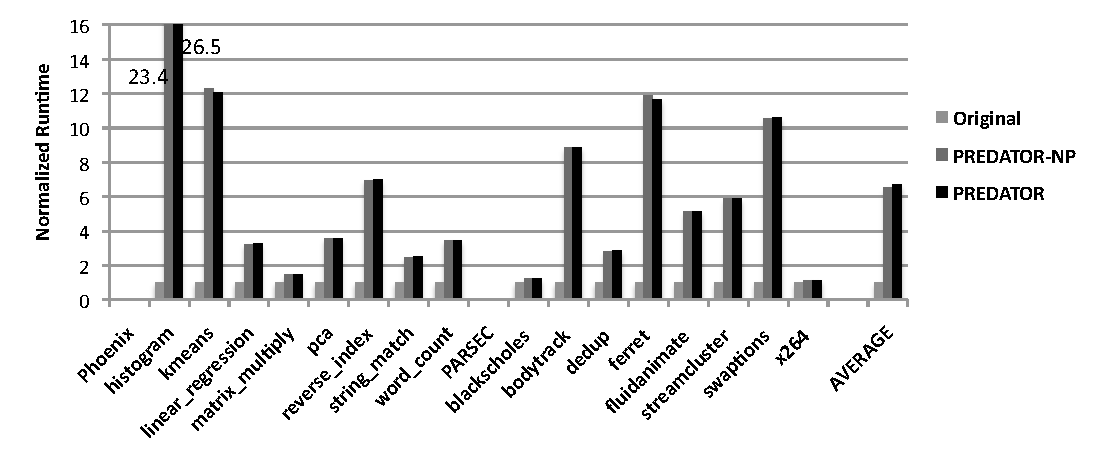
\includegraphics[width=6in]{predator/figure/perf}
\caption{
Performance overhead of \Predator{} with and without prediction(PREDATOR-NP).
\label{fig:perf}}
\end{figure*}

To avoid the effect caused by extreme outliers, all performance data shown in Figure~\ref{fig:perf} is based on the average of $10$ runs, excluding the maximum and minimum values. 

For $16$ benchmarks from the Phoenix and PARSEC benchmark suites and six real applications, \Predator{} imposes $5.4\times$ performance overhead. There is no noticeable difference on performance whether the prediction mechanism is enabled or not. 
 
Among these programs, five of them, histogram, kmeans, bodytrack, ferret, and swaptions, have more than $8\times$ performance overhead. The histogram benchmark runs more than $26\times$ slower than original executions with \pthreads{} library, because tracking detailed access on cache lines with false sharing exacerbates the false sharing effect (see more discussion in Section~\ref{sec:sample}).  For bodytrack and ferret, although there is no false sharing, \Predator{} detects a large amount of cache lines with writes larger than {\it Tracking-Threshold}. Thus, tracking those accessing details for those cache lines imposes significant performance overhead. Currently, we cannot identify the reasons why kmeans runs very slowly on \Predator{}.
   
\Predator{} imposes a small performance overhead for IO-bound applications, such as matrix\_multiply, blackscholes, x264, aget, Memcached, pbzip2, and pfscan, since \Predator{} does not add any performance overhead for IO operations.  

\subsection{Memory Overhead}
\label{sec:memoverhead}
We only evaluate the physical memory overhead of \Predator{}, instead of the virtual memory overhead, because \Predator{} allocates four gigabytes virtual memory for its custom memory allocator. Proportional set size (PSS) in \texttt{/proc/self/smaps} reflects the physical memory increase on the existing system of running an application~\cite{memusage}. Thus, we periodically collect this data and use the sum of different memory mappings as the total physical memory usage of running an application. We present the maximum value of physical memory usage in Figure~\ref{fig:memusage}. 

\Predator{} imposes less than 50\% memory overhead for 17 out of 22 applications.  For swaptions and aget, \Predator{} introduces more memory overhead because the original memory footprints of them are very small, only $3$ kilobytes. Adding the code of detection, prediction and reporting contributes to a large ratio of memory overhead. We are not clear why MySQL consumes much more memory than others. Although the average memory usage of all applications is over $2\times$, the total memory usage overhead is only about $40\%$ on \Predator{}. 


\subsection{Sensitivity to Different Sampling Rates}
\label{sec:sensitivity}
In Section~\ref{sec:sample}, we discuss that \Predator{} utilizes the sampling mechanism to reduce the tracking overhead. Running an application with different sampling rates does not affect its memory usage. Thus, we only evaluate the effect of different sampling rates on performance and effectiveness. 

The default sampling rate used by \Predator{} is 1\%. In this section, we also evaluate two other sampling rates, 0.1\% and 10\%. The performance results under the three different sample rates are shown in Figure~\ref{predator/figure:sample}. \Predator{} introduces less performance overhead under a lower sampling rate, which meets our expectation. Concerning effectiveness, even using the 0.1\% sampling rate, \Predator{} can still detect all false sharing problems, but with a lower number of cache invalidations. Thus, different sampling rates do not affect the detection effectiveness.
 
\begin{figure*}[!t]
\centering
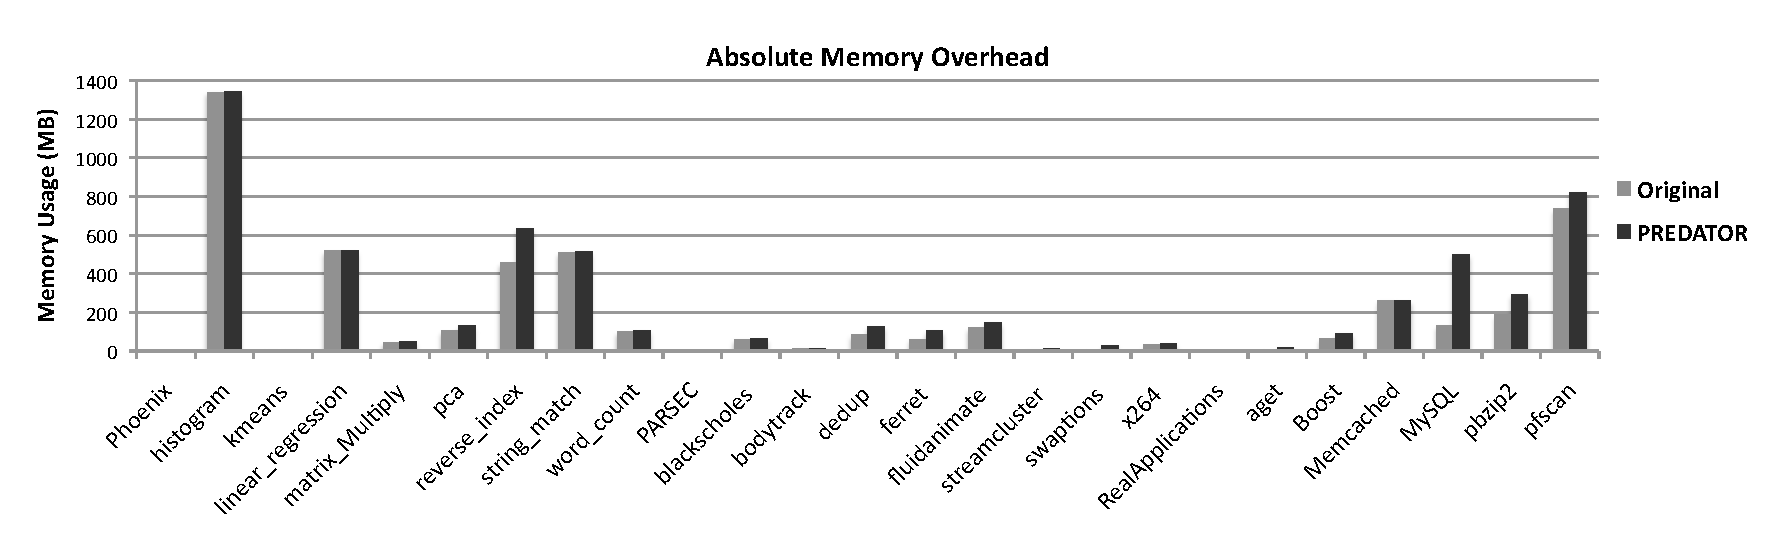
\includegraphics[width=6in]{predator/figure/absolutememory}
\caption{Absolute physical memory usage overhead with \Predator{}.}
\label{fig:absolutememusage}
\end{figure*}

\begin{figure*}[!t]
\centering
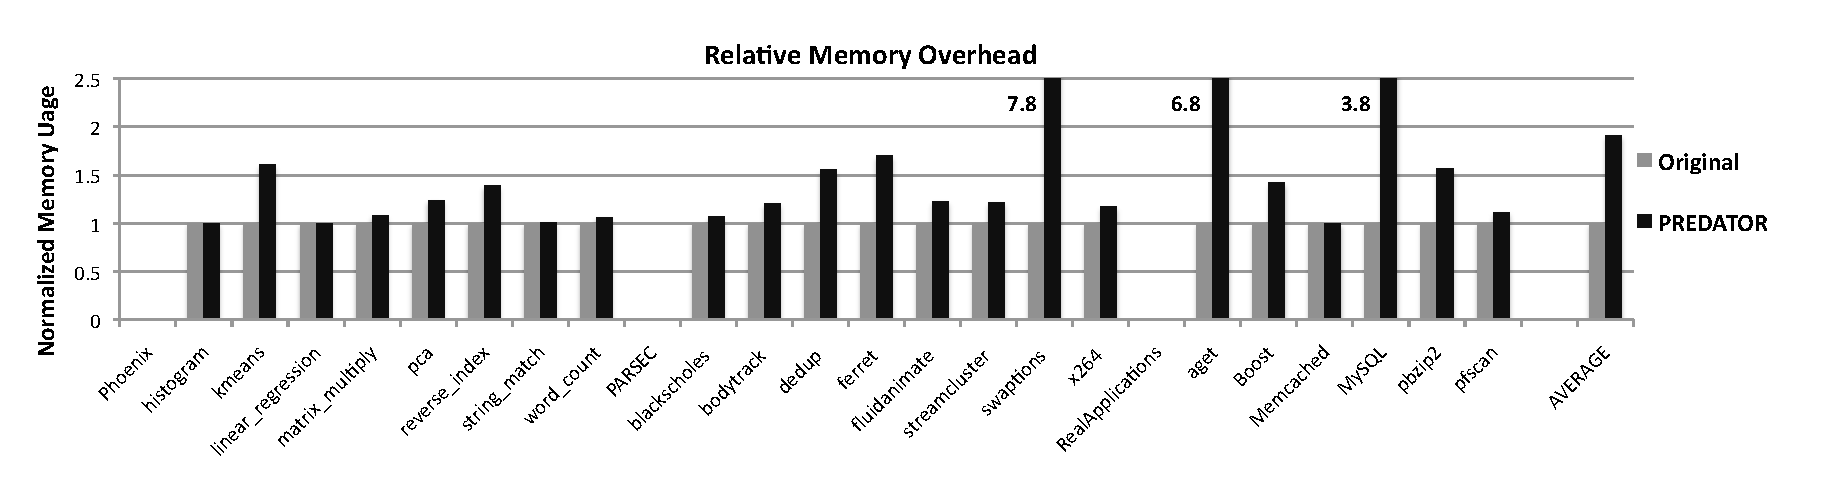
\includegraphics[width=6in]{predator/figure/memusage}
\caption{Relative physical memory usage overhead with \Predator{}.}
\label{fig:memusage}
\end{figure*}



\section{Discussion}
\label{sec:discussion}

This section analyzes some key limitations of \dthreads{} that
restrict its ability to run certain programs, limit the extent of
determinism it can guarantee, or potentially affect performance.


\textbf{Unsupported programs: }
\dthreads{} currently does not support programs with ad hoc
synchronizations, such as those that use atomic operations implemented in assembly.  However, the upcoming C++0X standard includes a library interface for atomic operations~\cite[pp. 1107--1128]{c++0xstandarddraft}, and a future version of \dthreads{} could correctly implement these by intercepting
these library calls and treating them as synchronization points. While
ad hoc synchronization is a common practice, it is also a notorious
source of bugs; Xiong et al.\ show that 22--67\% of the uses of ad hoc
synchronization lead to bugs or severe performance issues~\cite{ad-hoc-considered-harmful}.

\dthreads{} also currently does not write-share the stack
across threads, so that updates made by a thread to a stack variable
would not be reflected back to the parent, which could cause a program
to fail. Passing stack variables to a thread for modification is
extremely error-prone and generally deprecated, making this a rare
coding practice.

\textbf{External determinism: }
While \dthreads{} provides internal determinism, it does not
guarantee determinism when a program's behavior depends on external
sources of non-determinism, such as system time or I/O
events. Incorporation of \dthreads{} in the dOS framework, an OS
proposal that enforces system-level determinism, would provide full
deterministic execution, although this remains future
work~\cite{deterministic-process-groups}.

\textbf{Runtime performance: }
Section~\ref{sec:evaluation} shows that \dthreads{} can provide high
performance for a number of applications; in fact, for the majority of
the benchmarks examined, \dthreads{} matches or even exceeds the
performance of \pthreads{}. However, \dthreads{} could occasionally
degrade performance, sometimes substantially. One way it could do so
would be to exhibit an intensive use of locks (that is, acquiring and
releasing locks at high frequency), which are much more expensive
in \dthreads{} than in \pthreads{}. However, because of its determinism guarantees, \dthreads{} could allow programmers to greatly reduce their use of locks, and thus improve performance. Other application characteristics, also explored in Section~\ref{sec:performance}, can also impair performance
with \dthreads{}.


%  Since Surprise locking inside libraries. Not a limitation \emph{per
%  se} but definitely an issue that could surprise programmers.

% Draft can be downloaded from http://www.open-std.org/jtc1/sc22/wg21/docs/papers/2010/n3126.pdf.
%Fine once they are library calls, as they are in gcc and in the upcoming C++0X standard (cite!), since then we can intercept them.

\textbf{Memory consumption: }
Finally, because \dthreads{} creates private, per-process copies of
modified pages between commits, it can increase a program's memory
footprint by the number of modified pages between synchronization
points. This increased footprint does not seem to be a problem in
practice, both because the number of modified pages is generally far
smaller than the number of pages read, and because it is transitory:
all private pages are relinquished to the operating system
(via \texttt{madvise()}) at the end of every commit operation.

%Increased memory footprint (linear in the number of dirtied (modified) pages).




\section{Related Work}

\label{chapter:relatedwork}
This chapter first describes those related work to processes-as-threads framework and deterministic execution. Then it describes related work in false sharing detection, prevention, or both. 

\section{Processes-As-Threads framework}

BOP relies on strong isolation of processes to automatically and safely parallelize the execution of programs~\cite{DingBOP}. BOP forks a new process to do speculation, based on those pre-defined possibly parallel regions (PPR). In order to check the correctness, BOP tracks accesses on a page-based granularity. When there is no conflict and a speculative process reaches the end of its current PPR, its predecessor always commits its changes to the current process. However, BOP does not provide any synchronization support and can not be used to run normal multithreaded programs. 

Grace is a process-based approach designed to prevent
concurrency errors, such as deadlock, race conditions, and
atomicity errors by imposing a sequential semantics on
speculatively-executed threads~\cite{grace}. Grace supports only fork-join programs without inter-thread communication (e.g., condition variables or barriers), and rolls back threads when accesses of threads would violate sequential semantics: a thread accesses pages that have been accessed by its predecessors. Grace can not support arbitrary multithreaded programs. Similar to the Grace system, Sammati is a processes-as-threads system to detect and tolerate deadlock problems~\cite{Pyla:2010:ADA:1854273.1854288}. However, Sammati does not support the full range of synchronizations, without synchronizations, barriers, and signals. Also, Semmati can not avoid race conditions happening in creating twin pages, which are avoided by \Sheriff{} framework.

\begin{comment}
% Some usage of this framework
According to Revisions,  Grace cannot easily resolve all
conflicts on commit (like revisions do) and must thus restrict
tasks from producing such conflicts either statically (by type
system) or dynamically (pessimistic with blocking, or optimistic with abort and retry). Also, Grace allows only a restricted “fork-join” form of concurrency
Revisions~\ref{Burckhardt:2010:CPR:1869459.1869515}
\end{comment}

\section{Deterministic Multithreading}
The research on deterministic multithreading is a very active area these years. We describe some software-only, non- language-based approaches here.

\subsection{Software-only deterministic system}
Grace prevents deadlocks, race conditions, ordering and atomicity violations errors for those fork-join multithreaded programs by imposing a sequential semantics at join points~\cite{grace}. However, Grace does not support programs with interthread communications, such as conditional variables and barriers.

CoreDet is a compiler-based approach to 
support general-purpose multithreaded programs~\cite{Bergan:2010:CCR:1736020.1736029}. 
CoreDet instruments those memory read and write operations as long
as those operations can not be proved to be thread-local in static analysis. 
In the runtime phase, CoreDet divides the execution into 
alternating parallel and serial phases and guides all memory operations 
using a memory ownership table: only those owned locations can be accessed
in the parallel phases; all non-owned locations and synchronizations can only 
be accessed in the serial phases guided by a global token.
CoreDet guarantees deterministic execution for racy programs without memory errors,
but with very high performance overhead: 
averagely $3.5\times$ slower than those using \pthreads{} library.
In order to guarantee determinsim, 
CoreDet has to serialize \emph{all} external library calls without instrumentation.
CoreDet doesn not provide deterministic 
memory allocations, which can not guarantee determinism for programs with memory errors.  
% The use of synchronization points as commit boundaries also makes \dthreads{}
% code relatively \emph{robust}: when updates occur after a given number of 
% instructions retired (as in CoreDet and Kendo), it is impossible for 
% programmers to know when interleavings can occur. Such boundaries could vary 
% depending on the underlying architecture and would also be input-dependent, 
% meaning that slightly different inputs could lead to dramatically different
% thread interleavings. By contrast, \dthreads{} guarantees that only changes to
% the sequence of synchronization operations affect the order in which updates 
% are applied.
dOS~\cite{deterministic-process-groups} is an extension to CoreDet
that uses the same deterministic scheduling framework.  dOS 
supports deterministic communication for those threads and processes inside the same
deterministic process groups (DPGs) and handle those external non-determinism by recording and
replaying interactions across DPG boundaries. 

Determinator is a microkernel-based operating system that enforces
system-wide determinism~\cite{efficient-system-enforced}.
Determinator provides separate address spaces and supports interprocess
communications at explicit synchronizaton points. 
Determinator is a proof-of-concept system, which can not support the whole rage of
threads APIs and can not work on legacy programs.  

Some other works can only support limited determinism or need user annotation.
Kendo can only guarantee the determinism for race-free programs~\cite{1508256}. 
TERN~\cite{stable-deterministic} provides a best-effort system to 
apply memoized schedules for future runs with similar inputs. 
It can not guarantee the determinism for racy programs, as Kendo. 
Peregrine~\cite{peregrine:sosp11} is a system based on TERN, which tries to record
 memory accesses orders for racy portion and apply those schedules for future runs possibly.
However, both TERN and Peregrine do not support complete determinism (using a best effort)
and requires program annotations. 

\subsection{Hardware-related deterministic System}

\section{False Sharing}

This section describes related work in false sharing detection, prevention, or both. There is no previous
system to predict unobserved false sharing.

\subsection{False Sharing Detection}
Based on the SIMICS functional simulator, Schindewolf et al.\ designed a tool to report different kinds of cache usage information, such as cache misses and cache invalidations~\cite{falseshare:simulator}. Pluto relies on Valgrind dynamic instrumentation framework to track the sequence of memory read and write events on different threads, and reports a worst-case estimation of possible false sharing~\cite{falseshare:binaryinstrumentation1}.
Similarly, Liu uses Pin to collect memory access information, and reports total cache miss information~\cite{falseshare:binaryinstrumentation2}.
These tools impose about $100-200\times$ performance overhead.

Zhao et al.\ developed a tool based on DynamoRIO framework to detect false sharing and other cache contention problems
for multithreading programs~\cite{qinzhao}. 
It uses a shadow memory technique to maintain memory access history and detects cache invalidations based on the ownership of cache lines. However, it can only support at most $8$ threads. In addition, it cannot differentiate cold cache misses from actual false sharing problems.

Intel's performance tuning utility (PTU) uses Precise Event Based Sampling (PEBS) hardware support to detect false sharing problems ~\cite{detect:ptu, detect:intel}.  PTU cannot distinguish true sharing from false sharing. In addition, PTU aggregates memory accesses without considering memory reuses and access interleaving, leading to numerous false positives. Sanath et al. designed a machine learning based approach to detect false sharing problems. They train their classifier on mini-programs and apply this classifier to general programs ~\cite{mldetect}. Instead of instrumenting memory accesses, this tool relies on hardware performance counters to collect memory accesses events. It achieves very low performance overhead(about 2\%). But it relies on hardware support for its efficiency.  

In addition to their individual disadvantages,
all approaches discussed above share a common shortcoming:  
they cannot pinpoint the exact location of false sharing in the source code, so programmers have to examine the source code and identify problems manually.

Pesterev et al.\ present DProf, a tool that help programmers identify cache misses based on AMD's instruction-based sampling hardware~\cite{DProf}. DProf requires manual annotation to locate data types and object fields, and cannot detect false sharing when multiple objects reside on the same cache line.

\subsection{False Sharing Prevention}
\label{sec:fspreventwork}
% More approaches
Jeremiassen and Eggers use a compiler transformation to automatically adjust the memory layout of applications through padding and alignment~\cite{falseshare:compile}. Chow et al.\ alter parallel loop scheduling in order to avoid false
sharing~\cite{falseshare:schedule}. These approaches only works for regular, array-based scientific code.

Berger et al.\ describe Hoard, a scalable memory allocator that can reduce the possibility of false sharing by making different threads use different heaps~\cite{Hoard}. Hoard cannot avoid false sharing problem in global variables or within
a single heap object: the latter appears to be the primary source of real false sharing problems.

\subsection{False Sharing Detection and Prevention}

Plastic leverages the sub-page granularity memory remapping facility provided by the Xen hypervisor to detect and tolerate false sharing automatically~\cite{OSdetection}. However, the sub-page memory remapping mechanism is not currently supported by most existing operating system, reducing its generality. In addition, Plastic cannot pinpoint the exact source of false sharing.  
In order to utilize Plastic's prevention tool, a program has to run on the Xen hypervisor, limiting the applicability of their prevention technique.



% eliminate global lock
% possibly adopting a page-ownership protocol as used by ...

\section{Conclusion}
\label{sec:conclusion}

\dthreads{} is a deterministic replacement for the \pthreads{}
library that supports general-purpose multithreaded
applications. \dthreads{} is straightforward to deploy, requiring no
source code, and operates on commodity hardware. By converting threads
into processes, \dthreads{} leverages process isolation and virtual
memory protection to track and isolate concurrent memory updates with
low overhead. By committing these changes deterministically at natural
synchronization points in the code, rather than at boundaries based on
hardware performance counters, \dthreads{} not only ensures full
internal determinism---eliminating data races as well as
deadlocks---but does so in a way that is portable and easy to
understand. Its software architecture prevents false sharing, a
notorious performance problem for multithreaded applications running
on multiple, cache-coherent processors. The combination of these
approaches enables \dthreads{} to match or even exceed the performance
of \pthreads{} for the majority of the benchmarks examined here,
making \dthreads{} a safe and efficient alternative to \pthreads{} for
some applications.


\section{Acknowledgements}
\begin{comment}
We want to thank Qiang Zeng, Dinghao Wu and Peng Liu for providing
their test cases used in their Cruiser paper.  We also thank Scott Kaplan for his
suggestions and comments in the development of \doubletake{}.
\end{comment}

{
\bibliographystyle{abbrv}
\bibliography{refs}
}

\end{document}
